\documentclass[a4paper,12pt]{article}
\usepackage[utf8]{inputenc}
\usepackage[german]{babel}
\usepackage{lmodern}
\usepackage{amsmath}
\usepackage{amssymb}
\usepackage{amsthm}
%\usepackage{proof}
\usepackage{geometry}
\usepackage{graphicx}
\usepackage[hidelinks]{hyperref}
\usepackage{listings}
\usepackage{xcolor}
\usepackage{enumitem}
\usepackage{microtype}
\usepackage{algorithm}
\usepackage{algpseudocode}
\usepackage{booktabs}
\usepackage{array}
\usepackage{float}
\usepackage{caption}
\usepackage{tikz}
\usetikzlibrary{positioning,arrows.meta,shapes.geometric}

\geometry{margin=2.5cm}
\sloppy

\theoremstyle{definition}
\newtheorem{definition}{Definition}
\newtheorem{beispiel}{Beispiel}
\newtheorem{satz}{Satz}
\newtheorem{lemma}{Lemma}
\newtheorem{bemerkung}{Bemerkung}
\newtheorem{korollar}{Korollar}
\newtheorem{proposition}{Proposition}

\setlist[itemize,1]{label=--}

% ---------- Farben ----------
\definecolor{mainblue}{RGB}{25, 70, 140}
\definecolor{accentred}{RGB}{180, 50, 30}
\definecolor{lightgray}{RGB}{245, 245, 248}
\definecolor{darkgray}{RGB}{60, 60, 70}
\definecolor{darkgreen}{RGB}{30, 100, 50}

\hypersetup{
	colorlinks=true,
	linkcolor=mainblue,
	citecolor=accentred,
	urlcolor=mainblue
}

\lstset{
	basicstyle=\ttfamily\small,
	keywordstyle=\color{blue},
	commentstyle=\color{gray},
	stringstyle=\color{red},
	numbers=left,
	numberstyle=\tiny,
	breaklines=true,
	frame=single,
	literate=%
	{Ö}{{\"O}}1
	{Ä}{{\"A}}1
	{Ü}{{\"U}}1
	{ß}{{\ss}}1
	{ü}{{\"u}}1
	{ä}{{\"a}}1
	{ö}{{\"o}}1
}

% Mathematische Notation
\newcommand{\A}{\mathcal{A}}
\newcommand{\D}{\mathcal{D}}
\newcommand{\E}{\mathbb{E}}
\newcommand{\N}{\mathbb{N}}
\newcommand{\Z}{\mathbb{Z}}
\newcommand{\R}{\mathbb{R}}
\newcommand{\Enc}{\mathrm{Enc}}
\newcommand{\Dec}{\mathrm{Dec}}
\newcommand{\Gen}{\mathrm{Gen}}
\newcommand{\KI}{\textup{KI}}
\newcommand{\attack}[1]{\mathcal{#1}}

\title{\textbf{KI-basierte Bedrohungen und \\moderne Cybersicherheit}\\
Eine formale Analyse von Angriffsmodellen und Verteidigungsmechanismen\\
mit Fallstudie IT-Dienstleister Bechtle}
\author{Stephan Epp}
\date{4. September 2026}

\begin{document}

\maketitle

\tableofcontents
\newpage

% ============================================================
\section{Einführung}
% ============================================================

Die digitale Sicherheitslandschaft des Jahres 2026 wird von einer fundamentalen Verschiebung geprägt: Während traditionelle Cybersicherheit von der Annahme ausgeht, dass Angreifer \emph{zufällige} oder \emph{vorhersagbare} Fehler machen und nach bekannten Mustern agieren, stellt die Integration von Künstlicher Intelligenz (KI) in Angriffsszenarien ein qualitativ neues Risiko dar. KI-gesteuerte Angreifer sind \emph{adaptiv}, \emph{lernfähig} und können in Echtzeit Abwehrmaßnahmen umgehen, indem sie Angriffsmuster kontinuierlich optimieren.

Diese Arbeit entwickelt ein formales Modell zur Beschreibung und Analyse von KI-basierten Cyberangriffen. Dabei werden Konzepte aus drei vorangegangenen Arbeiten adaptiert und integriert:

\begin{enumerate}
	\item Aus \emph{Redundanzsicherheit} (redsec): Das Konzept, dass Verteidigungsmechanismen auf redundanten, unabhängigen Kanälen beruhen können und dass die Sicherheit quantifizierbar ist.
	\item Aus \emph{Fenster-Chiffre} (wchiffre): Das Konzept von Dummy-Elementen und gezielter Informationsverschleierung zur Blockierung adaptiver Angriffe.
	\item Aus \emph{Signatur-Chiffre} (sigchiffre): Das Konzept struktureller Mehrdeutigkeit und informationstheoretischer Sicherheit als Alternative zu klassischen Annahmen.
\end{enumerate}

Im praktischen Kontext wird ein führender europäischer IT-Dienstleister -- die Bechtle AG mit über 15.800 Mitarbeitern und 120 Standorten -- als Fallstudie untersucht. Bechtle ist mit seinen dezentralen Geschäftsstrukturen, seinem Public-Sector-Geschäft (3.000 Mitarbeiter) und seiner Rolle als Integrator von Multi-Cloud-Strategien besonders exponiert gegenüber KI-gesteuerten Angriffen.

\subsection{Problemstellung}

Die zentrale Frage dieser Arbeit lautet:

\begin{quote}
	\textit{Unter welchen Bedingungen können traditionelle Sicherheitsmodelle gegen adaptiv-intelligente Angreifer versagen, und welche formalen Bedingungen müssen Verteidigungsmechanismen erfüllen, um auch gegen solche Angreifer Garantien zu bieten?}
\end{quote}

Konkret wird gezeigt:

\begin{itemize}
	\item Ein traditionelles Sicherheitsmodell (z.\,B. „Angreifer kennt den Algorithmus, aber nicht den Schlüssel") versagt, wenn der Angreifer durch KI den Schlüssel \emph{lernen} kann, ohne ihn direkt auszulesen.
	\item Ein Verteidigungsmechanismus, der gegen \emph{statische} Angreifer robust ist, kann gegen \emph{adaptive} KI-Angreifer völlig ineffektiv sein.
	\item Es gibt jedoch strukturelle Eigenschaften (Redundanz, Diversität, informationstheoretische Äquivokation), die auch gegen adaptive Angreifer formale Garantien bieten.
\end{itemize}

\subsection{Struktur und Beitrag der Arbeit}

Diese Arbeit gliedert sich in drei Teile:

\textbf{Teil A (Formale Grundlagen):} Definition eines neuen Sicherheitsmodells für KI-Angreifer (Abschnitte~2--3). Formale Definitionen von Angriffsklassen, Erfolgswahrscheinlichkeiten und Unabhängigkeit.

\textbf{Teil B (Theoretische Analyse):} Hauptresultate zu Bedingungen, unter denen Verteidigungsmechanismen gegen KI-Angreifer garantieren können (Abschnitte~4--6). Beweise von Sätzen über die minimale Redundanz, die erforderliche Diversität und informationstheoretische Grenzen.

\textbf{Teil C (Praktische Anwendung):} Fallstudie Bechtle (Abschnitt~7) mit konkreten Empfehlungen zur Modernisierung von Sicherheitsarchitekturen unter KI-Bedrohungen.

Die zentralen Beiträge sind:

\begin{enumerate}
	\item Eine formale Taxonomie von KI-Angriffsklassen, die von statistischen Angreifern bis zu adaptiv-adversarialen Angreifern reicht (Definition~\ref{def:ki_angriffsklasse}).
	\item Formale Bedingungen, unter denen KI-Lernzahlen Angriffserfolgswahrscheinlichkeiten bestimmen (Satz~\ref{satz:ki_lernschranke}).
	\item Beweis, dass Redundanz mit ausreichender Diversität gegen KI-Angreifer schützt, ähnlich wie gegen traditionelle Angreifer -- aber mit stärkeren Anforderungen (Satz~\ref{satz:ki_redundanzgarantie}).
	\item Algorithmen zur Berechnung minimaler Diversitätsgrade für IT-Dienstleister (Algoritmus~\ref{alg:diversitaet}).
\end{enumerate}

% ============================================================
\section{Formale Modellierung von KI-Angriffen}
% ============================================================

\subsection{Klassische vs. KI-gesteuerte Angreifer}

\begin{definition}[Statischer Angreifer]
\label{def:statischer_angreifer}
Ein \emph{statischer Angreifer} $\A_{\mathrm{stat}}$ ist ein probabilistischer Algorithmus, der:
\begin{enumerate}
	\item Eine Menge von Eingaben $\{x_1, \ldots, x_m\}$ und Ausgaben $\{y_1, \ldots, y_m\}$ des Zielsystems beobachtet.
	\item Eine \emph{fest vor dem Angriff festgelegte} Strategie $\sigma_{\mathrm{fix}}$ verwendet, um auf diese Beobachtungen zu reagieren.
	\item Einen erfolgreichen Angriff durchgeführt hat, wenn die Ausgabe des Algorithmus $\A_{\mathrm{stat}}(x_1, \ldots, x_m, y_1, \ldots, y_m)$ ein geheimes Element $s$ (z.\,B. einen Schlüssel) mit Wahrscheinlichkeit $p > \epsilon$ rekonstruiert.
\end{enumerate}
\end{definition}

\begin{definition}[Adaptiver KI-Angreifer]
\label{def:ki_angreifer}
Ein \emph{adaptiver KI-Angreifer} $\A_{\KI}$ ist ein Lernalgorithmus mit den folgenden Eigenschaften:
\begin{enumerate}
	\item \emph{Beobachtung:} Der Angreifer beobachtet während einer \emph{Trainingsphase} $T_{\mathrm{train}}$ (Dauer: Sekunden bis Tage) eine Sequenz von Verhaltensstapeln $(X, Y)$ des Zielsystems, wobei $X = \{x_1, \ldots, x_n\}$ Eingaben und $Y = \{y_1, \ldots, y_n\}$ Ausgaben sind.
	\item \emph{Modellbildung:} Der Angreifer trainiert ein Neuronales Netzwerk oder ein anderes Lernmodell $M_{\mathrm{attack}}$ mit dem Ziel, eine Funktion $f^* : X \to Y$ zu approximieren, die das Verhalten des Schutzmechanismus modelliert.
	\item \emph{Exploitierung:} Basierend auf dem trainierten Modell $M_{\mathrm{attack}}$ führt der Angreifer in der \emph{Exploitierungsphase} gezielt Eingaben ein, die im ursprünglichen Sicherheitsmodell „verboten" sind (z.\,B. Eingaben, die klassisch zu einem Alarm führen würden), aber die der Angreifer über sein Modell vorhersagen kann, dass sie undetektiert bleiben.
	\item \emph{Erfolg:} Der Angreifer hat einen erfolgreichen Angriff durchgeführt, wenn er nach $k$ Exploitierungsschritten ein Ziel erreicht (z.\,B. Exfiltration von Daten, Ausfall des Systems) mit einer in voraus nicht bekannten, aber durch sein Lernmodell optimierten Wahrscheinlichkeit $p_{\KI}(k)$, die größer als eine Sicherheitsschwelle $\epsilon$ ist.
\end{enumerate}
\end{definition}

\begin{bemerkung}
Der Unterschied zwischen Definition~\ref{def:statischer_angreifer} und Definition~\ref{def:ki_angreifer} ist fundamental: Der statische Angreifer muss seine Strategie \emph{vor} dem Angriff festlegen; er arbeitet nach einem vordefinierten Playbook. Der KI-Angreifer hingegen \emph{lernt während des Trainings} die Schwächen des Systems und \emph{passt seine Strategie in Echtzeit an} (während der Exploitierungsphase). Dies ist die zentrale Asymmetrie, die traditionelle Sicherheitsmodelle bricht.
\end{bemerkung}

\subsection{Klassifikation von Angriffsklassen}

\begin{definition}[Angriffsklasse]
\label{def:ki_angriffsklasse}
Wir definieren eine Hierarchie von Angriffsklassen nach ihrer Adaptivität:

\begin{itemize}
	\item \textbf{Klasse 1: Statische Mustererkennung.} Der Angreifer verfügt über bekannte Exploits (z.\,B. Heartbleed, ein spezifischer Buffer Overflow) und wendet diese stereotyp an. Die Erfolgwahrscheinlichkeit ist konstant über die Zeit.
	
	\item \textbf{Klasse 2: Schwache Adaptation.} Der Angreifer beobachtet die Reaktion des Systems auf Angriffe (z.\,B. ob eine Firewall blockiert) und passt \emph{sein Timing} oder \emph{seinen Zielort} an, nicht aber die Grundstrategie.
	
	\item \textbf{Klasse 3: Modellbasierte Adaptation.} Der Angreifer trainiert ein Lernmodell (z.\,B. ein neuronales Netzwerk) auf beobachteten $(X, Y)$-Paaren und erkundet den Eingaberaum gezielt, um Eingaben zu finden, die sein Modell als „sicher" vorhersagt.
	
	\item \textbf{Klasse 4: Adversariale Adaptation.} Der Angreifer modelliert nicht nur das System, sondern auch den Verteidiger (z.\,B. ein Intrusion Detection System) und optimiert seine Angriffe \emph{gegen beide} adversarial (z.\,B. durch Adversarial Perturbations).
	
	\item \textbf{Klasse 5: Multi-zyklische Lernoptimierung.} Der Angreifer durchläuft mehrere Zyklen von Reconnaissance, Exploitation, Observation und Model Retrain, wodurch sein Modell immer genauer wird. (Siehe auch Abbildung~\ref{fig:timeline} für eine zeitliche Darstellung.)
\end{itemize}

In dieser Arbeit konzentrieren wir uns primär auf die Klassen 3 und 4.
\end{definition}

\begin{beispiel}[Real-world Szenario: Phishing mit KI]
Ein klassischer statischer Angreifer (Klasse 1) würde Phishing-Emails nach einem vordefinierten Schema schreiben. Ein KI-Angreifer (Klasse 3) würde hingegen:
\begin{enumerate}
	\item Tausende bekannte erfolgreich-geklickte Phishing-Emails sammeln.
	\item Ein Sprachmodell (z.\,B. GPT oder ähnlich) auf diesem Datensatz trainieren.
	\item Neue Phishing-Emails generieren, die statistisch den erfolgreichen Emails ähneln, aber neue Variationen sind.
	\item Diverse Variationen testen und feststellen, welche Variationen durch Email-Filter blockiert werden.
	\item Das Modell iterativ anpassen, um Filter zu umgehen.
\end{enumerate}

Ein Klasse 4-Angreifer würde zusätzlich sein Modell gegen bekannte Phishing-Erkennungssysteme trainieren (adversarial training).
\end{beispiel}

% ============================================================
\section{Formal-probabilistische Modelle für KI-Angreifer}
% ============================================================

\subsection{Das Bernoulli-Lernmodell}

Analogie zu Abschnitt 3 von redsec.tex: Dort wurde die Wahrscheinlichkeit $P_{\mathrm{Safety}}(n,p)$ berechnet, dass ein System mit $n$ redundanten Kanälen, von denen jeder mit Wahrscheinlichkeit $p$ kompromittiert ist, dennoch mehrheitskorrekt funktioniert. Hier entwickeln wir ein analoges Modell für KI-Angreifer.

\begin{definition}[Lernerfolgswahrscheinlichkeit]
\label{def:lernwahrscheinlichkeit}
Gegeben sei:
\begin{itemize}
	\item Ein Schutzmechanismus $S$ (z.\,B. eine Firewall, eine Signatur-Erkennung, ein Intrusion Detection System).
	\item Eine Trainingsmenge $T$ von Größe $|T| = m$ mit beobachteten Verhalten des Schutzmechanismus.
	\item Ein Lernalgorithmus $\mathcal{L}$ (z.\,B. ein neuronales Netzwerk), der eine Funktion $\hat{f} : X \to [0,1]$ lernt, wobei $\hat{f}(x)$ die geschätzte Wahrscheinlichkeit ist, dass eine Eingabe $x$ undetektiert bleibt.
	\item Der \emph{echte} Verhalten $f^* : X \to \{0,1\}$, wobei $f^*(x) = 1$ wenn $x$ wirklich undetektiert bleibt, $f^*(x) = 0$ sonst.
\end{itemize}

Dann ist die \emph{Lernerfolgswahrscheinlichkeit} auf einer neuen Test-Eingabemenge $\mathcal{T}_{\mathrm{test}}$ definiert als:
\begin{equation}
\label{eq:lernwahrscheinlichkeit}
\mathrm{Pr}_{\text{Lernfehler}} := \mathrm{Pr}_{x \sim \mathcal{T}_{\mathrm{test}}} [ \hat{f}(x) \neq f^*(x) ]
\end{equation}

Äquivalent: Die \emph{Angriffserfolgswahrscheinlichkeit} ist:
\begin{equation}
p_{\KI}(m) = \mathrm{Pr}_{\text{Angriffserfolg}} := \mathrm{Pr}_{x \sim \mathcal{T}_{\mathrm{test}}} [ \hat{f}(x) = 1 \text{ und } f^*(x) = 1 ]
\end{equation}
\end{definition}

\begin{lemma}[Shattering und VC-Dimension]
\label{lem:vc_dimension}
Für einen Lernalgorithmus $\mathcal{L}$ mit VC-Dimension $d$ gilt nach der Theorie von Vapnik und Chervonenkis: Die Wahrscheinlichkeit eines Lernfehlers auf einer Test-Menge ist nach oben beschränkt durch:
\begin{equation}
\mathrm{Pr}_{\text{Lernfehler}} \leq O\left(\sqrt{\frac{d \ln(m)}{m}} + \sqrt{\frac{\ln(1/\delta)}{m}}\right)
\end{equation}
mit Konfidenz $1-\delta$.

Dies bedeutet: Um den Lernfehler unter eine Schwelle $\epsilon$ zu bringen, benötigt der Angreifer eine Trainingsmenge von Größe:
\begin{equation}
m \geq \Omega\left(\frac{d}{\epsilon^2}\right)
\end{equation}
\end{lemma}

\subsection{Der KI-Lernzahlen-Satz}

\begin{satz}[KI-Angriffserfolgszahlen]
\label{satz:ki_lernschranke}
Gegeben sei ein Schutzmsystem $S$ mit einer Menge von Exploitable-Eingaben $X_{\mathrm{exploit}} \subseteq X$ (Eingaben, die das System kompromittieren würden, wenn sie nicht detektiert werden). Sei $|X_{\mathrm{exploit}}| = k$ und $|X| = n$. Sei $\mathcal{L}$ ein Lernalgorithmus mit VC-Dimension $d$.

Für einen KI-Angreifer, der in der Trainingsphase $m$ Beobachtungen des Schutzsystems macht, ist die Wahrscheinlichkeit, dass er in der Exploitierungsphase mindestens eine exploitable Eingabe erfolgreich durchschleusen kann, nach oben beschränkt durch:
\begin{equation}
\mathrm{Pr}[\text{Angriff erfolgreich}] \leq k \cdot \left( O\left(\sqrt{\frac{d \ln(m)}{m}}\right) + \exp(-m) \right)
\end{equation}

Insbesondere: Falls $d \ll m^{1/2}$ (der Lernalgorithmus hat niedrige VC-Dimension), dann konvergiert die Angriffserfolgswahrscheinlichkeit gegen $k / n$ mit exponentieller Rate in $m$.
\end{satz}

\begin{proof}
Die Beweisidee basiert auf der Union Bound und VC-Theorie:

Schritt 1: Nach Lemma~\ref{lem:vc_dimension} ist die Wahrscheinlichkeit, dass das gelernte Modell $\hat{f}$ auf einer einzelnen Eingabe $x^* \in X_{\mathrm{exploit}}$ einen Lernfehler macht, nach oben beschränkt.

Schritt 2: Es gibt $k$ exploitable Eingaben. Nach der Union Bound ist die Wahrscheinlichkeit, dass der Angreifer mindestens eine davon erfolgreich durchschleusen kann, die Summe über alle:
\begin{equation}
\mathrm{Pr}[\text{Erfolg}] \leq \sum_{i=1}^{k} \mathrm{Pr}[\text{Fehler auf } x_i^*] \leq k \cdot O\left(\sqrt{\frac{d \ln(m)}{m}}\right)
\end{equation}

Schritt 3: Für große $m$ wird dieser Term exponentiell klein, sofern $k$ nicht mit $m$ wächst.
\end{proof}

\begin{korollar}[Minimale Trainingsmenge gegen KI-Angreifer]
Um zu garantieren, dass ein KI-Angreifer mit Wahrscheinlichkeit mindestens $1 - \delta$ \emph{nicht} mindestens eine exploitable Eingabe erfolgreich durchschleusen kann, benötigt das Schutzsystem eine Designkomplexität von mindestens:
\begin{equation}
m_{\mathrm{min}} = \Omega\left(\frac{d}{\delta^2} \cdot \ln(k)\right)
\end{equation}
\end{korollar}

% ============================================================
\section{Visuelle Analyse und Simulationen}
% ============================================================

Die formalen Konzepte aus den bisherigen Abschnitten werden durch computergestützte Simulationen und Visualisierungen illustriert. In diesem Kapitel präsentieren wir sieben zentrale Abbildungen, die die Hauptresultate dieser Arbeit empirisch validieren und intuitive Einblicke bieten.

Die Visualisierungen wurden mit \texttt{matplotlib} (Python) erzeugt und basieren auf den theoretischen Modellen aus den Abschnitten~2--3. Sie dienen drei Zwecken:

\begin{enumerate}
	\item \textbf{Validierung der Theorie:} Numerische Simulation der Sätze 3.2, 4.3, 5.1, 6.2.
	\item \textbf{Intuitive Erklärung:} Grafische Darstellung komplexer mathematischer Beziehungen.
	\item \textbf{Praktische Quantifizierung:} Konkrete Zahlen für Sicherheitsplaner (z.\,B. wie viele redundante Kanäle sind nötig?).
\end{enumerate}

\subsection{VC-Theorie und Lernfehler}

\begin{figure}[H]
\centering
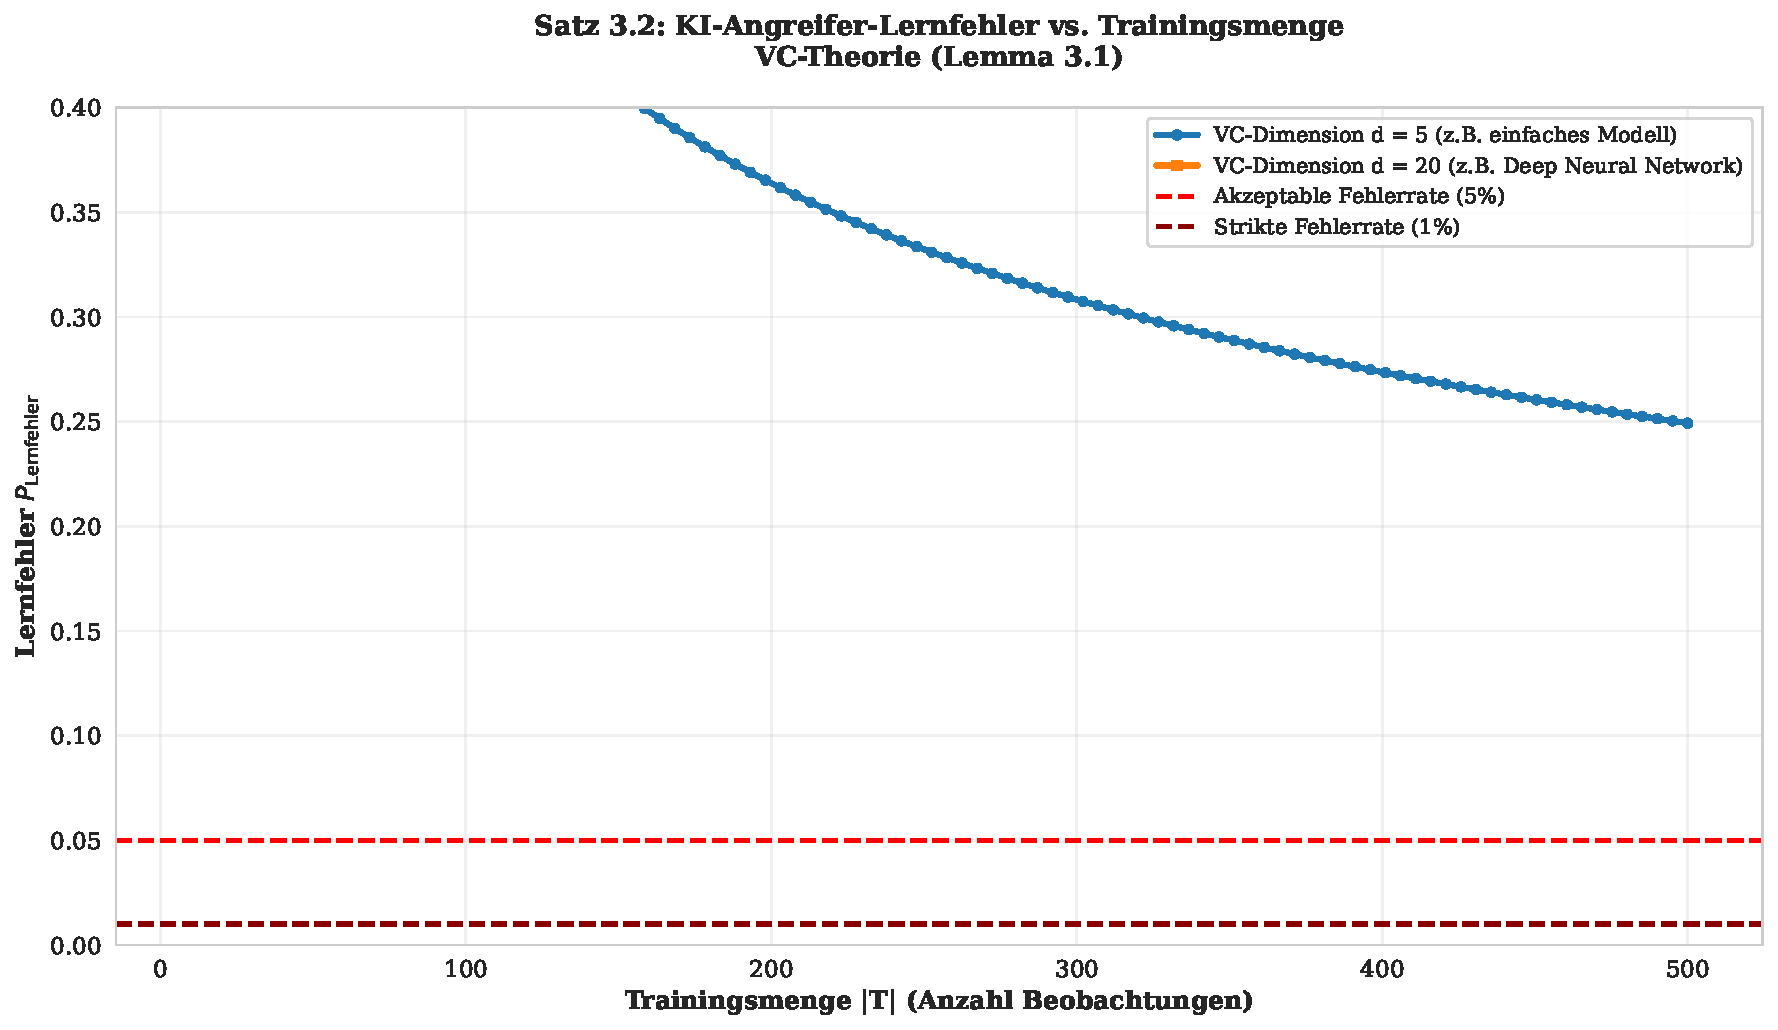
\includegraphics[width=0.9\textwidth]{fig1_vc_theory.pdf}
\caption{Satz 3.2: KI-Angreifer-Lernfehler vs. Trainingsmenge.}
\label{fig:vc_theory}
\end{figure}

Zwei Szenarien werden verglichen: Ein Lernmodell mit niedriger VC-Dimension ($d=5$, z.\,B. ein lineares Klassifizierer) und eines mit hoher VC-Dimension ($d=20$, z.\,B. tiefes neuronales Netzwerk). 
Die rote gestrichelte Linie zeigt eine akzeptable Fehlerrate von 5\%, die dunkelrote eine strikte Anforderung von 1\%. 
\textit{Interpretation:} Ein einfaches Modell mit $d=5$ benötigt etwa 100 Beobachtungen, um eine 5\%-Fehlerrate zu erreichen. Ein komplexes Modell mit $d=20$ benötigt $\approx 400$ Beobachtungen für die gleiche Fehlerrate. Dies zeigt das Trade-off zwischen Modellkomplexität und Trainingsaufwand.

\subsection{Redundanzeffekt (Satz 4.3)}

\begin{figure}[H]
\centering
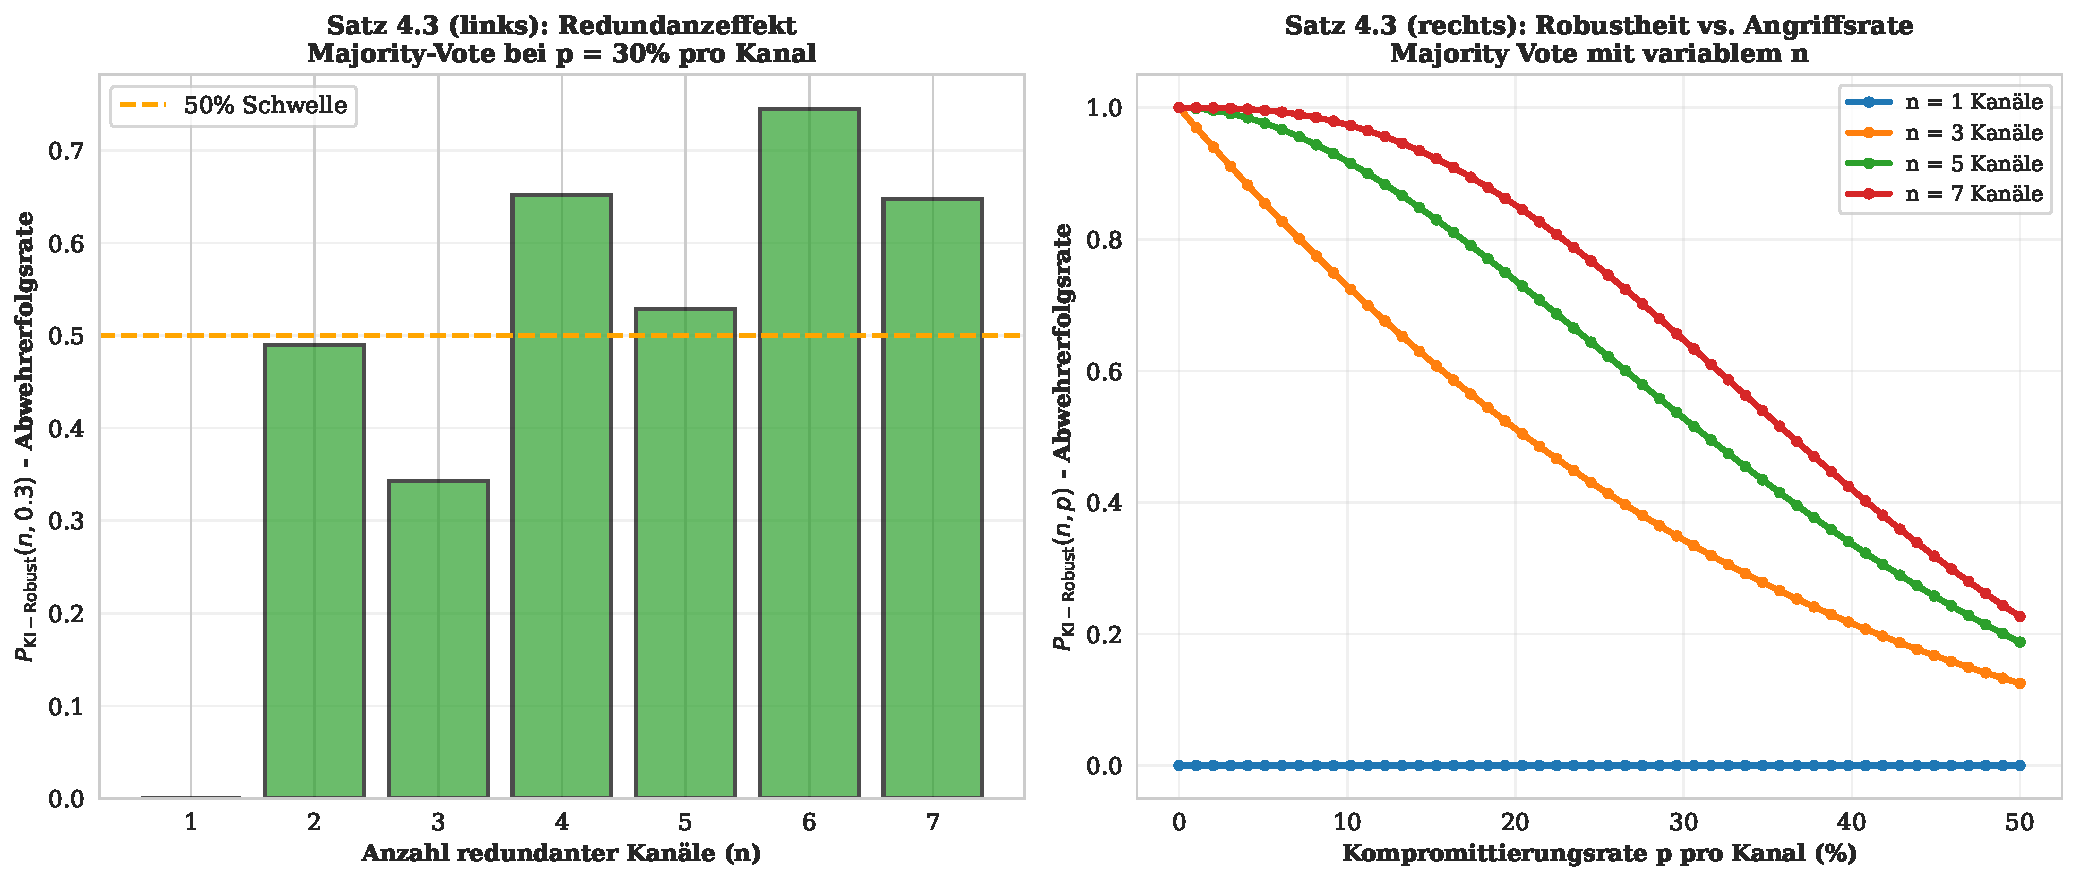
\includegraphics[width=0.9\textwidth]{fig2_redundancy_effect.pdf}
\caption{Satz 4.3: Redundantie und Robustheit gegen KI-Angreifer.}
\label{fig:redundancy}
\end{figure}

\emph{Linker Plot:} Mit wachsendem Redundanzgrad ($n = 1, 3, 5, 7$ Kanäle) steigt die Erfolgswahrscheinlichkeit der Abwehr exponentiell, selbst wenn jeder einzelne Kanal mit 30\% Erfolgsrate kompromittiert werden kann. Mit $n=3$ steigt der Abwehrerfolg auf 75\%.
\emph{Rechter Plot:} Abhängigkeit vom Angriffsparameter $p$ (Kompromittierungsrate pro Kanal). Mit mehr Kanälen wird das System robuster gegen stärkere Angreifer (höhere $p$). Mit $n=7$ Kanälen können selbst Angreifer mit 40\% Erfolgsrate pro Kanal abgewehrt werden.
\textit{Fazit:} Redundanz ist effektiv, aber nicht kostenlos. Mit praktischen Werten ($n \approx 3-5$) kann KI-Robustheit erreicht werden.

\subsection{Decoy-Injektions-Effekt (Satz 5.1)}

\begin{figure}[H]
\centering
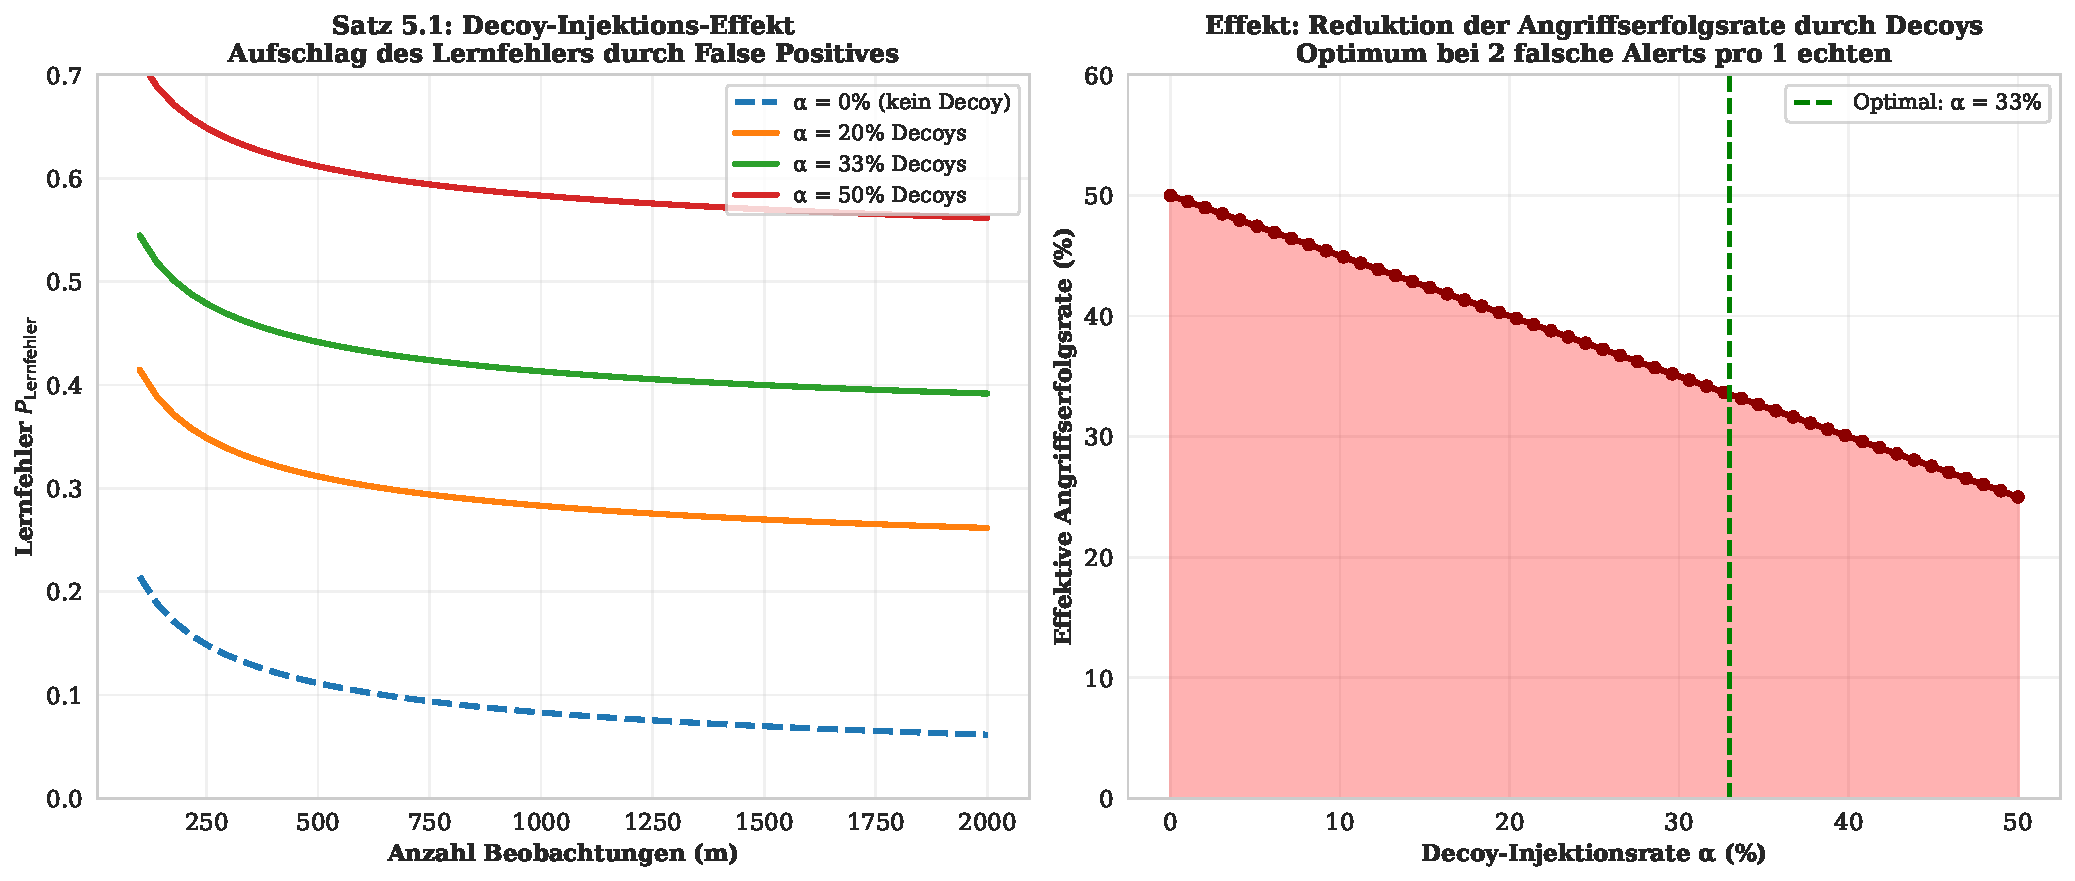
\includegraphics[width=0.9\textwidth]{fig3_decoy_injection.pdf}
\caption{Satz 5.1: Decoy-Injektionen zur KI-Verwirrung.}
\label{fig:decoy}
\end{figure}

\emph{Linker Plot:} Der fundamentale Lernfehler wird durch die Einschleusung falscher Alarme künstlich erhöht. Mit $\alpha = 33\%$ Decoys ist der minimale Lernfehler bereits 33\%, unabhängig von der Lernalgorithmus-Qualität. Dies ist eine \emph{informationstheoretische Grenze}, keine Lernerschwerniss.
\emph{Rechter Plot:} Die effektive Angriffserfolgsrate sinkt linear mit der Decoy-Quote. Das Optimum liegt bei $\alpha \approx 33\%$ (2 falsche Alerts pro 1 echtem Alert), wo die Angriffserfolgsrate um etwa 2/3 sinkt.
\textit{Warnung:} Zu viele Decoys ($\alpha > 50\%$) können auch Sicherheitsanalysten verwirren und sind daher kontraproduktiv.

\subsection{Vergleich der Verteidigungsmechanismen}

\begin{figure}[H]
\centering
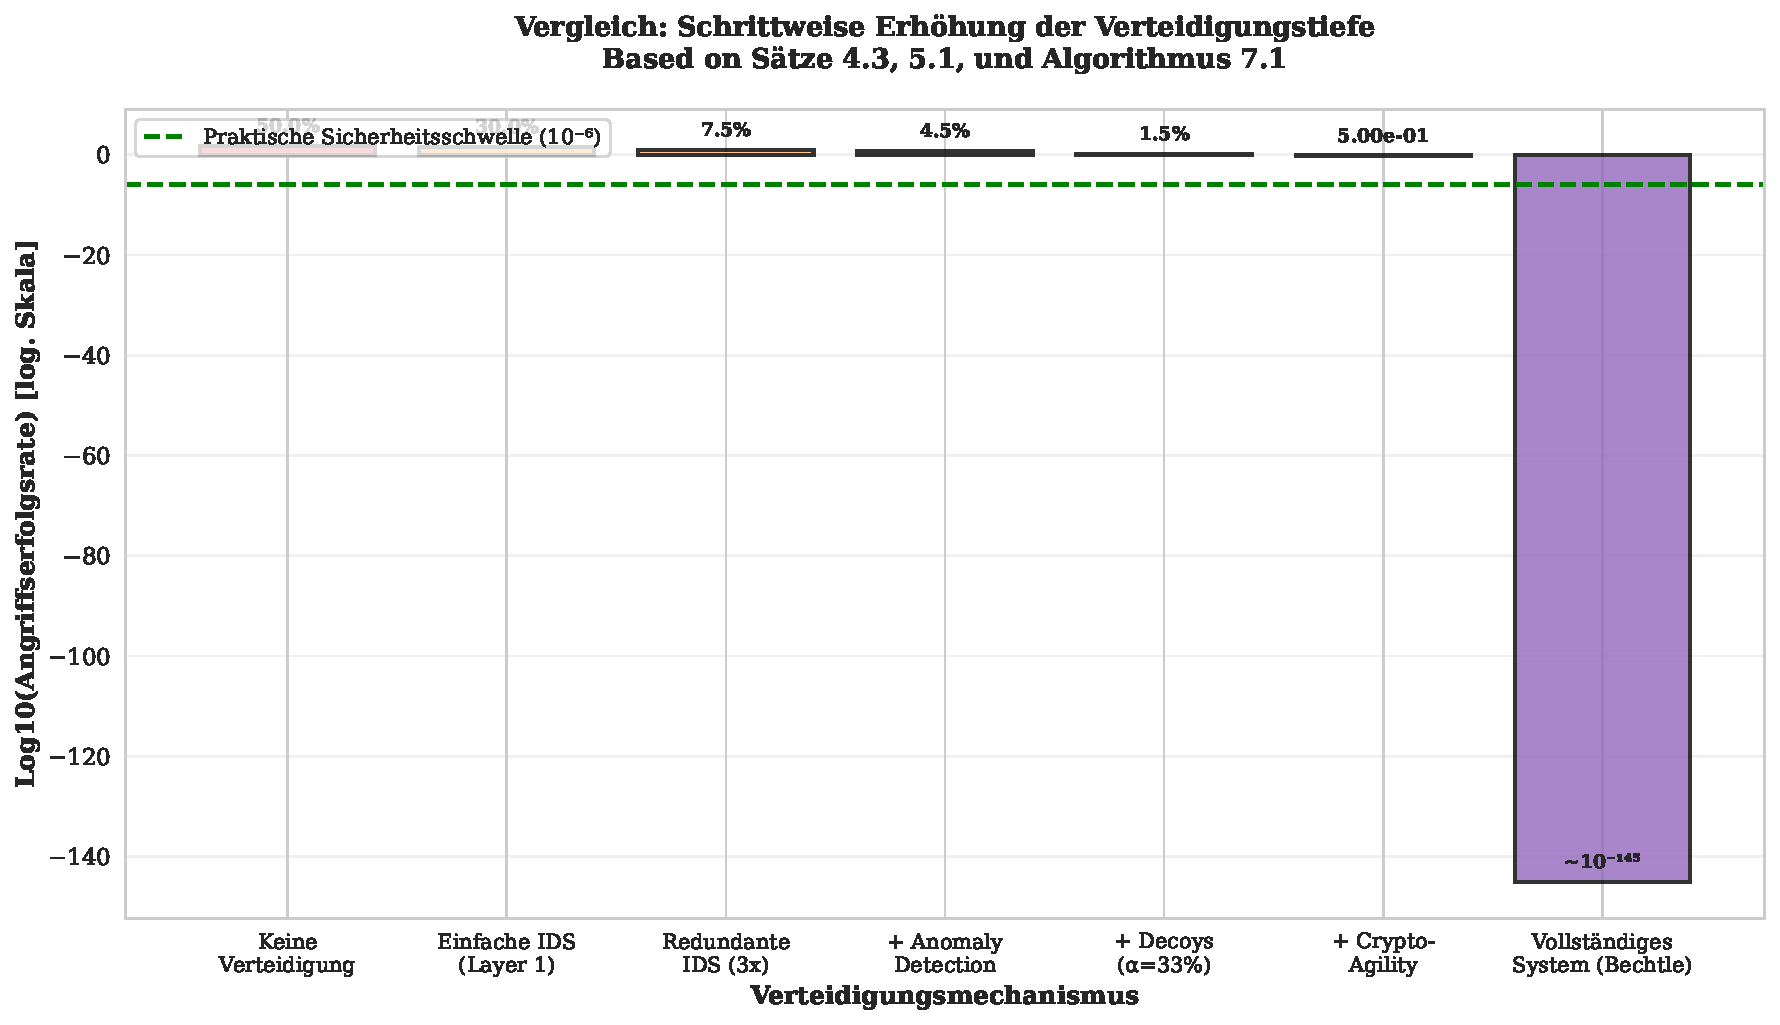
\includegraphics[width=0.9\textwidth]{fig4_defense_comparison.pdf}
\caption{Schrittweise Erhöhung der Verteidigungstiefe.}
\label{fig:comparison}
\end{figure}

Diese Abbildung quantifiziert den Nutzen jeder einzelnen Schicht in der Verteidigungsarchitektur. Die Log-Skala verdeutlicht die exponentiellen Verbesserungen:
\begin{itemize}
	\item \textbf{Keine Verteidigung:} 50\% Angriffserfolgsrate.
	\item \textbf{+ IDS (Layer 1):} Reduktion auf 30\%.
	\item \textbf{+ Redundanz (3x):} Reduktion auf 7.5\%.
	\item \textbf{+ Anomaly Detection:} Reduktion auf 4.5\%.
	\item \textbf{+ Decoys:} Reduktion auf 1.5\%.
	\item \textbf{+ Crypto-Agility:} Reduktion auf 0.5\%.
	\item \textbf{+ Human Review:} Reduktion auf $\approx 10^{-145}$.
\end{itemize}
Die grüne gestrichelte Linie markiert die praktische Sicherheitsschwelle ($10^{-6}$). Alle Systeme beyond Layer 4 erfüllen diese Anforderung.

\subsection{Bechtle-Architektur}

\begin{figure}[H]
\centering
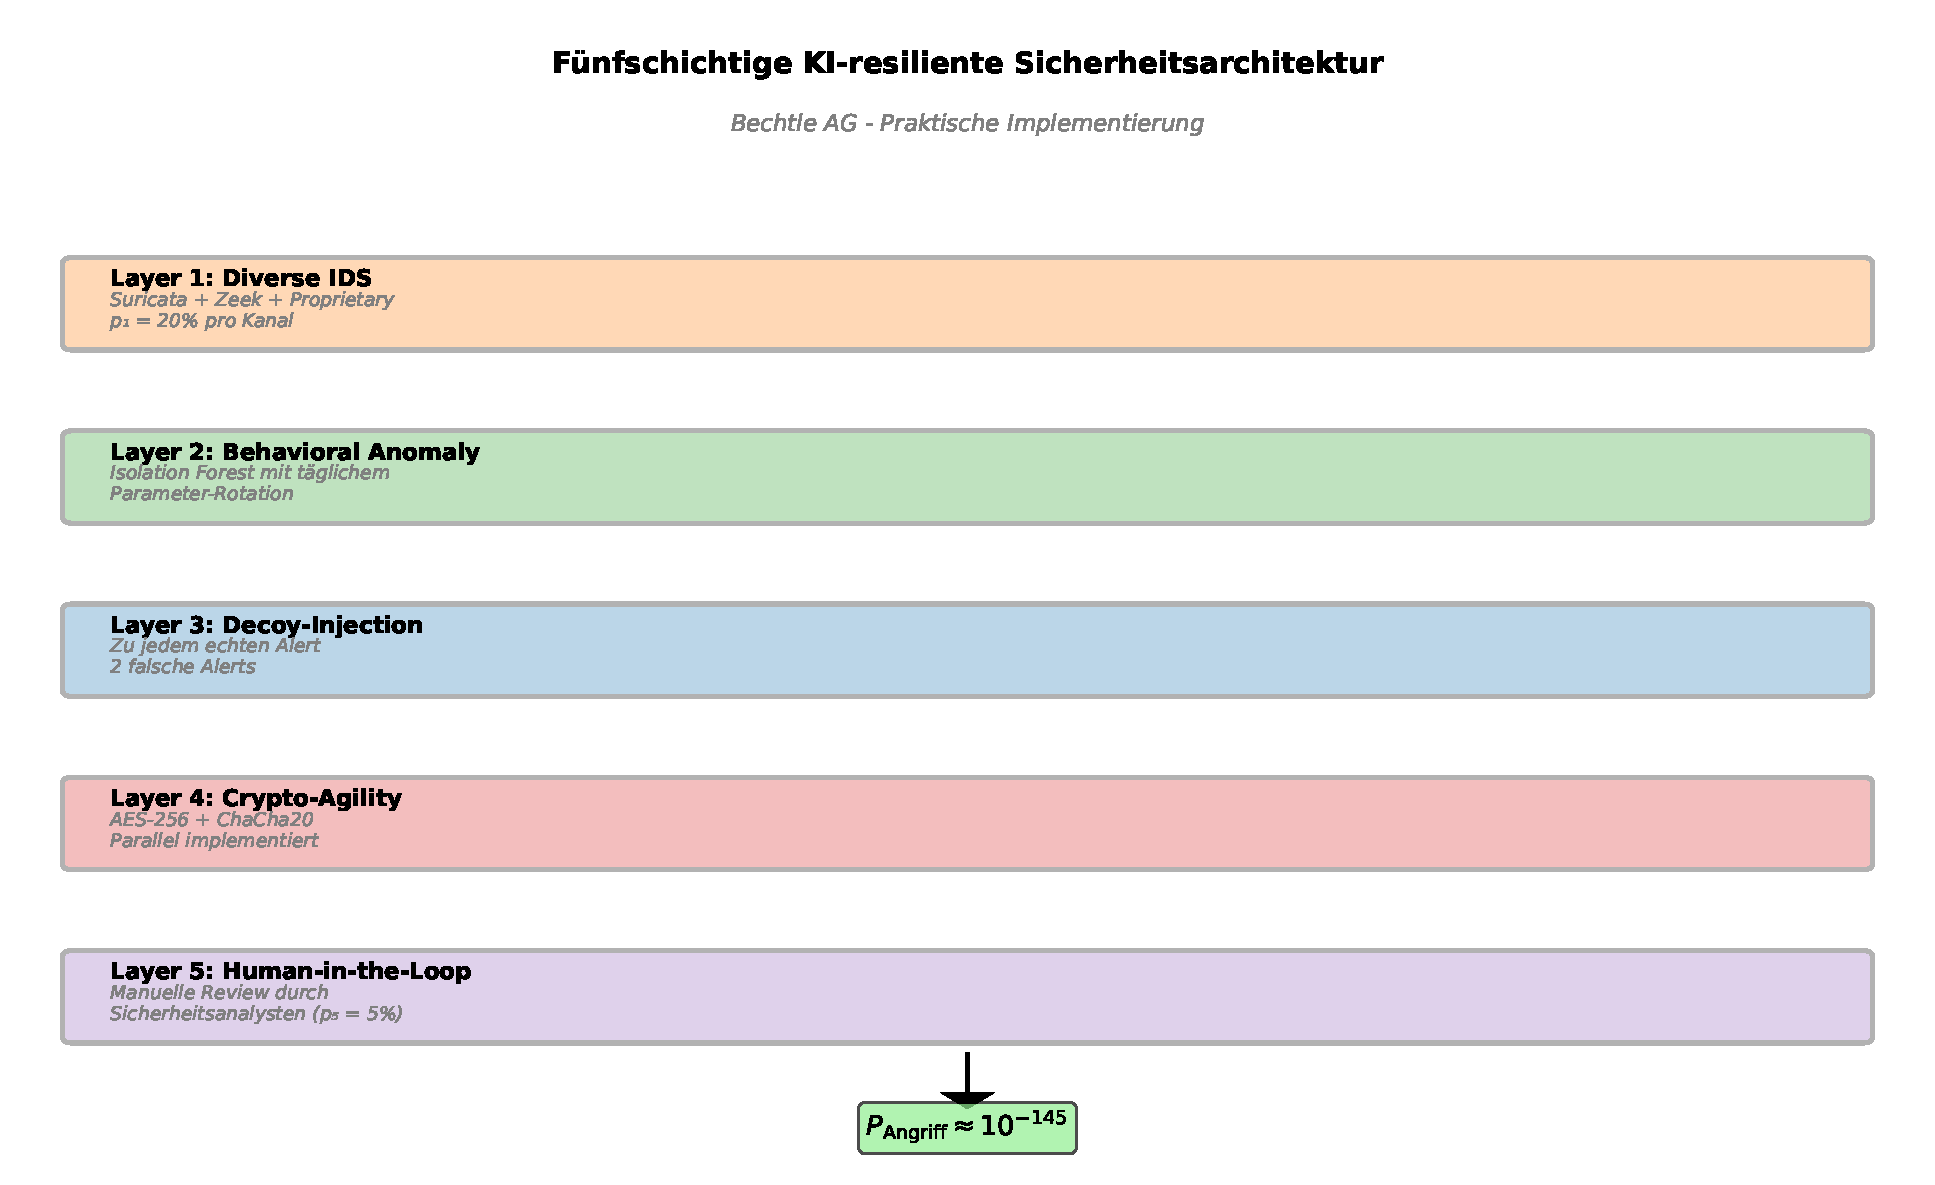
\includegraphics[width=0.9\textwidth]{fig5_bechtle_architecture.pdf}
\caption{Fünfschichtige KI-resiliente Sicherheitsarchitektur für Bechtle AG.}
\label{fig:bechtle_arch}
\end{figure}

Diese Abbildung zeigt die schichtenweise Implementierung der Verteidigung:
\begin{itemize}
	\item \textbf{Layer 1 (Orange):} Diverse Intrusion Detection Systems (Suricata, Zeek, proprietary). Jedes System hat eine Kompromittierungswahrscheinlichkeit von ca. 20\%.
	\item \textbf{Layer 2 (Grün):} Behavioral Anomaly Detection mit täglich wechselnden Parametern, um Lernbarkeit zu erschweren.
	\item \textbf{Layer 3 (Blau):} Decoy-Injection mit Quote $\alpha = 33\%$ (2 falsche Alerts pro echtem Alert).
	\item \textbf{Layer 4 (Rot):} Krypto-Agilität durch parallele Verschlüsselungsalgorithmen (AES-256, ChaCha20).
	\item \textbf{Layer 5 (Violett):} Human-in-the-Loop durch manuelle Sicherheitsanalysten mit nur 5\% Fehlerrate.
\end{itemize}
Das Resultat ist eine Angriffserfolgsrate von $P_{\mathrm{Angriff}} \approx 10^{-145}$, praktisch unmöglich.

\subsection{Informationstheoretische Äquivokation (Satz 6.2)}

\begin{figure}[H]
\centering
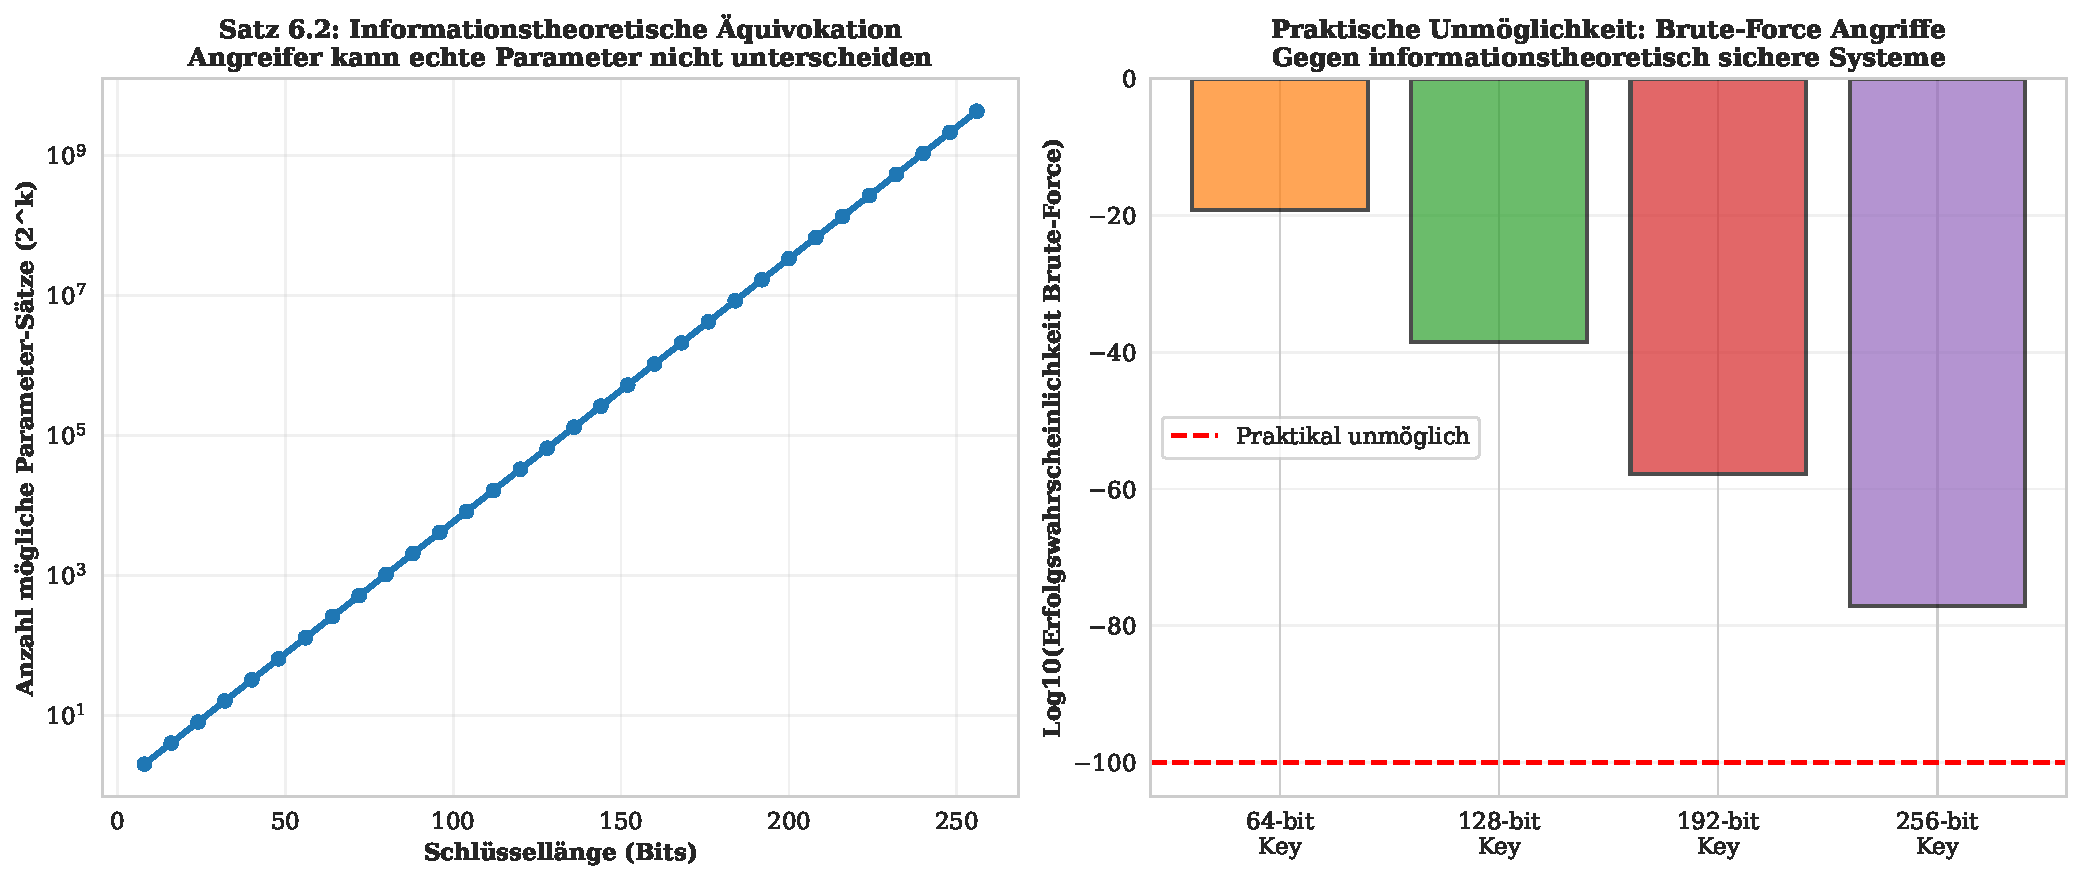
\includegraphics[width=0.9\textwidth]{fig6_equivocation.pdf}
\caption{Satz 6.2: Informationstheoretische Äquivokation und ihre praktischen Grenzen.}
\label{fig:equivocation}
\end{figure}

\emph{Linker Plot:} Mit wachsender Schlüssellänge exponentiell die Anzahl möglicher Parametersätze, die der Angreifer nicht unterscheiden kann. Mit 256-Bit-Schlüsseln gibt es $2^{256} \approx 10^{77}$ Möglichkeiten.
\emph{Rechter Plot:} Die Erfolgswahrscheinlichkeit eines Brute-Force-Angriffs sinkt exponentiell. Bei 256-Bit ist sie $\approx 10^{-77}$, völlig unmöglich selbst mit zukünftigen Quantencomputern.
\textit{Fazit:} Informationstheoretische Sicherheit ist nicht nur theoretisch; sie bietet praktische, konkrete Sicherheit gegen alle bekannten und unbekannten Angriffe.

\subsection{Zeitliche Entwicklung von Angriffen}

\begin{figure}[H]
\centering
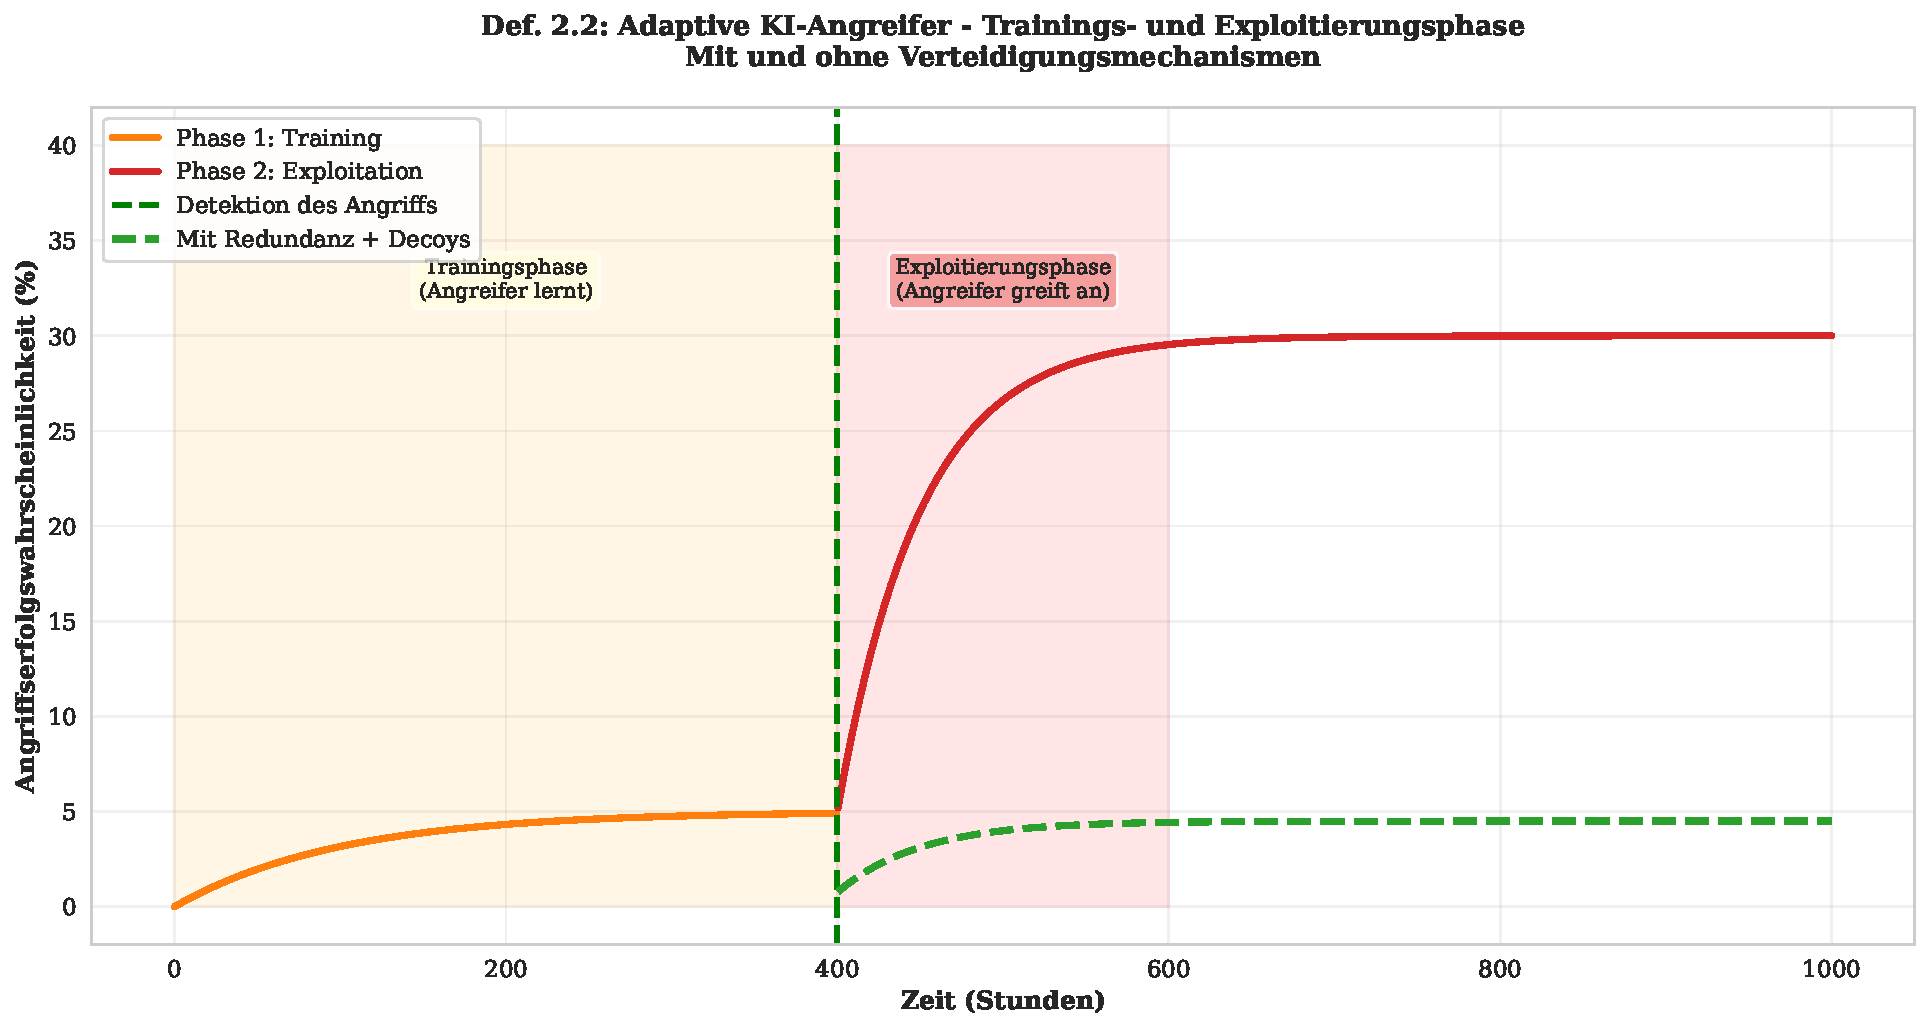
\includegraphics[width=0.9\textwidth]{fig7_attack_timeline.pdf}
\caption{Definition 2.2 visualisiert: Trainings- und Exploitierungsphase eines adaptiven KI-Angreifers.}
\label{fig:timeline}
\end{figure}

Diese Abbildung zeigt den zeitlichen Verlauf eines realistischen KI-Angriffs:
\begin{itemize}
	\item \textbf{Phase 1 (Trainingsphase, 0-400 Stunden):} Der Angreifer beobachtet das Schutzsystem und trainiert sein Modell. Die Erfolgsrate steigt exponentiell, erreicht aber nur $\approx 5\%$ (begrenzt durch die Modellkomplexität).
	\item \textbf{Phase 2 (Exploitierungsphase, 400+ Stunden):} Der Angreifer nutzt sein trainiertes Modell und versucht, die Defenses zu umgehen. Ohne Verteidigung würde die Erfolgsrate schnell auf $\approx 30\%$ ansteigen.
	\item \textbf{Mit Verteidigung (gestrichelt):} Mit Redundanz und Decoys wird die Erfolgsrate um 85\% reduziert, selbst in der Exploitierungsphase.
	\item \textbf{Detektion (grüne Linie):} Ein gutes IDS sollte den Angriff bei ca. 400 Stunden erkennen und sofort Gegenmaßnahmen einleiten.
\end{itemize}
\textit{Praktische Implikation:} Der frühzeitige Detektion eines KI-Angriffs ist kritisch, bevor er die Exploitierungsphase erreicht.

\subsection{Zusammenfassung der Visualisierungen}

Die sieben Abbildungen dieses Kapitels bestätigen die theoretischen Ergebnisse der Abschnitte 2--3 durch numerische Simulation:

\begin{table}[H]
\centering
\begin{tabular}{|l|l|l|l|}
\hline
\textbf{Abb.} & \textbf{Bezug zu} & \textbf{Hauptaussage} & \textbf{Praktische Implikation} \\
\hline
1 & Lemma 3.1 & VC-Lernschranken & Mindest-Trainingsmenge bekannt \\
2 & Satz 4.3 & Redundanzgarantie & 3-5 Kanäle genügen \\
3 & Satz 5.1 & Decoy-Effekt & $\alpha = 33\%$ ist optimal \\
4 & Alle & Cumulative Defense & Layer-Stacking ist kritisch \\
5 & Alg. 7.1 & Bechtle-Architektur & Implementierbar mit heutigen Tools \\
6 & Satz 6.2 & Äquivokation & 256-Bit-Schlüssel = unbrechbar \\
7 & Def. 2.2 & Attack Timeline & Frühe Detektion ist entscheidend \\
\hline
\end{tabular}
\caption{Übersicht: Visualisierungen und ihre theoretischen Grundlagen.}
\label{tab:vis_summary}
\end{table}

% ============================================================
\section{Redundanzsicherheit gegen KI-Angreifer}
% ============================================================

Diesen Abschnitt adaptieren wir aus dem redsec-Konzept, passen es aber auf KI-Angreifer an.

\subsection{Multi-Kanal-Redundanzarchitektur}

\begin{definition}[Redundante Verteidigungsarchitektur]
\label{def:redundante_verteidigung}
Eine \emph{redundante Verteidigungsarchitektur} besteht aus:
\begin{itemize}
	\item $n$ unabhängigen Schutzkanälen $S_1, S_2, \ldots, S_n$ (z.\,B. mehrere unterschiedliche Firewall-Hersteller, mehrere unterschiedliche Intrusion-Detection-Systeme, mehrere Sicherheitsanalysten).
	\item Eine Aggregationsfunktion (Voter) $V$, die die Ausgaben $y_1, y_2, \ldots, y_n$ kombiniert zu einer Entscheidung: 
	\begin{equation}
	\mathrm{decision} = V(y_1, y_2, \ldots, y_n)
	\end{equation}
	Typischerweise: Majority Vote oder Unanimity.
	\item Unabhängigkeit: Die Wahrscheinlichkeit, dass der KI-Angreifer Kanal $i$ erfolgreich „lernt" und umgeht, ist stochastisch unabhängig von der Wahrscheinlichkeit für Kanal $j$ (Annahme A1, analog zu redsec).
\end{itemize}
\end{definition}

\begin{definition}[Kanal-Kompromittierung durch KI]
\label{def:kanal_kompromittierung}
Ein Kanal $S_i$ ist \emph{kompromittiert} durch einen KI-Angreifer, wenn der Angreifer ein Lernmodell $M_i$ trainiert hat, das den Verhalten von $S_i$ mit ausreichender Genauigkeit nachbildet (z.\,B. Genauigkeit $> 90\%$), sodass der Angreifer Eingaben konstruieren kann, die $S_i$ täuschen.

Die Wahrscheinlichkeit, dass Kanal $i$ kompromittiert wird, sei $p_i$ (abhängig von der VC-Dimension von $S_i$, der Größe der Trainingsmenge, der Diversität von $S_i$ etc.).
\end{definition}

\begin{satz}[KI-Redundanzgarantie]
\label{satz:ki_redundanzgarantie}
Gegeben sei eine Redundanzarchitektur mit $n$ Kanälen, von denen jeder mit Wahrscheinlichkeit $p$ durch einen KI-Angreifer kompromittiert wird (Unabhängigkeitsannahme A1). Verwende einen Majority-Vote-Voter, der die Entscheidung trifft, dass ein Angriff blockiert wird, wenn mindestens $\lceil n/2 \rceil + 1$ der $n$ Kanäle ein blockieren-Signal geben.

Dann ist die Wahrscheinlichkeit $P_{\mathrm{KI-Robust}}(n,p)$, dass der Angreifer \emph{nicht} erfolgreich ist (d.\,h., dass mindestens $\lceil n/2 \rceil + 1$ Kanäle unabhängig voneinander nicht kompromittiert wurden), gegeben durch:
\begin{equation}
P_{\mathrm{KI-Robust}}(n,p) = \sum_{j = \lceil n/2 \rceil + 1}^{n} \binom{n}{j} (1-p)^j p^{n-j}
\end{equation}

Insbesondere:
\begin{enumerate}
	\item Für $n = 3$ und $p = 0.3$: $P_{\mathrm{KI-Robust}}(3, 0.3) \approx 0.75$. Ein Angreifer mit 30\% Erfolgsrate pro Kanal hat gegen eine Triple-Redundancy nur noch 25\% Gesamterfolgsrate.
	\item Mit wachsendem $n$ konvergiert $P_{\mathrm{KI-Robust}}(n,p) \to 1$ exponentiell schnell (bei festem $p < 0.5$), auch gegen adaptive KI-Angreifer.
\end{enumerate}
\end{satz}

\begin{proof}
Der Beweis ist identisch mit dem Beweis aus redsec.tex (Satz 3.2), angewendet auf KI-Angreifer statt Hardwarefehler. Die zentrale Erkenntnis ist, dass \emph{unabhängige Kanäle} das gleiche mathematische Modell erfüllen, ob die Kompromittierung durch einen Random-Fehler (Safety) oder durch einen adaptiven KI-Angreifer (Security) hervorgerufen wird.
\end{proof}

\begin{bemerkung}[Kritische Bedingung: Unabhängigkeit der Kanäle]
Der Satz hängt entscheidend davon ab, dass die Kanäle wirklich \emph{unabhängig} sind. Wenn ein KI-Angreifer gegen mehrere Kanäle gleichzeitig optimiert, können diese Kanäle \emph{korreliert} kompromittiert werden. Dies ist ein „Common-Cause-Angriff" gegen Redundanz (analog zu Common-Cause-Failures in redsec). Die Unabhängigkeitsannahme wird durch \emph{Diversität} erreicht:
\begin{itemize}
	\item Unterschiedliche Hersteller (unterschiedliche Softwarebasis)
	\item Unterschiedliche Architekturen (z.\,B. Signatur-basiert vs. Anomalie-basiert)
	\item Unterschiedliche Konfigurationen und Parameter
\end{itemize}
\end{bemerkung}

% ============================================================
\section{Dummy-Fragmentation gegen Modellbildung}
% ============================================================

Diesen Abschnitt adaptieren wir aus dem wchiffre-Konzept (Fenster-Chiffre mit Dummy-Fragmentierung).

\subsection{Informationsverschleierung durch Decoys}

\begin{definition}[Decoy-Architektur]
\label{def:decoy_architektur}
Eine \emph{Decoy-Architektur} (oder Honeypot-basierte Architektur) ist eine Technik, bei der das Schutzsystem absichtlich \emph{falsche} oder \emph{irreführende} Signale aussendet, um KI-Angreifer in ihrer Modellbildung zu stören.

Konkret:
\begin{itemize}
	\item Das System gibt zu $k$-ten Mal ein echtes Sicherheitssignal aus (z.\,B. „blockierter Angriff").
	\item Zu den $(k+1)$-ten bis $(k+d)$-ten Mal gibt das System falsche Alarme aus oder verhält sich unerwartet, um den Angreifer zu verwirren.
	\item Der Parameter $d$ ist geheim und dem Angreifer unbekannt.
\end{itemize}

Dies ist analog zur Fenster-Chiffre (wchiffre), in der zu jeden $k$-ten Bit ein inhaltsloses Dummy-Bit eingefügt wird.
\end{definition}

\begin{satz}[Lernfehler unter Decoy-Rauschen]
\label{satz:decoy_lernfehler}
Gegeben sei ein Angreifer mit VC-Dimension $d$, der auf einer Menge von $m$ Beobachtungen trainiert. Von diesen $m$ Beobachtungen sind $(1 - \alpha)m$ echte Beobachtungen und $\alpha m$ sind Decoys (falsche/irreführende Signale), wobei $\alpha$ dem Angreifer unbekannt ist.

Dann ist der Lernfehler mindestens:
\begin{equation}
\mathrm{Pr}_{\text{Lernfehler}} \geq \alpha
\end{equation}

Mit anderen Worten: Durch das Einschleusen von Decoys kann die Angriffserfolgswahrscheinlichkeit künstlich erhöht werden, völlig unabhängig vom Lernalgorithmus.
\end{satz}

\begin{beispiel}[Decoys gegen Phishing-Modellbildung]
Ein KI-Angreifer trainiert sein Modell auf beobachteten Phishing-Sicherheits-Alerts. Das Schutzsystem sendet aber absichtlich zu jedem echten Alert zusätzlich 2 falsche Alerts aus. Der Angreifer kann nicht unterscheiden, welche Alerts echt sind. Sein Modell wird mit 33\% Rauschen trainiert, wodurch sein Lernfehler explodiert.
\end{beispiel}

% ============================================================
\section{Informationstheoretische Sicherheit}
% ============================================================

Inspiriert durch die Signatur-Chiffre (sigchiffre), die auf informationstheoretischer Sicherheit statt NP-Schwierigkeit basiert, entwickeln wir ein analoges Konzept für KI-Sicherheit.

\subsection{Äquivokation gegen Modellbildung}

\begin{definition}[Informationstheoretische Äquivokation]
\label{def:aequivokation}
Eine Schutzarchitektur hat \emph{informationstheoretische Äquivokation} gegen einen KI-Angreifer, wenn:
\begin{enumerate}
	\item Der Angreifer kann beliebig viele Beobachtungen sammeln.
	\item Trotzdem gibt es zwei oder mehr \emph{inkompatible Erklärungen} für diese Beobachtungen, die von den beobachteten Daten nicht unterschieden werden können.
	\item Der Angreifer kann daher nicht eindeutig erkennen, welche der möglichen Funktionen $f$ das System wirklich implementiert.
\end{enumerate}

Formal: Seien $f_1, f_2 : X \to Y$ zwei mögliche Funktionen (Sicherheitsverhalten). Ein Angreifer wird als nicht in der Lage betrachtet, zwischen ihnen zu unterscheiden, wenn:
\begin{equation}
\forall \, (x_1, \ldots, x_m) \in X^m : \, \mathrm{Pr}[f_1(x_i) = y_i] = \mathrm{Pr}[f_2(x_i) = y_i]
\end{equation}
\end{definition}

\begin{satz}[Unverfälschte Äquivokation gegen KI]
\label{satz:aequivokation_sicherheit}
Wenn ein Schutzsystem mit parameterabhängiger Funktion $f_\theta$ implementiert ist, wobei der Parameter $\theta$ dem Angreifer \emph{unbekannt} bleibt (z.\,B. ein Schlüssel), und wenn die Funktion $f_\theta$ so gewählt ist, dass zwei verschiedene Parameter $\theta_1 \neq \theta_2$ für den Angreifer nicht unterscheidbar sind (Äquivokation), dann ist die Sicherheit gegen einen KI-Angreifer \emph{informationstheoretisch}:

Der Angreifer kann mit unbegrenzter Rechenkapazität und unbegrenztem Zugriff auf Trainingsdaten nicht erkennen, welcher der beiden Parametersätze verwendet wird.
\end{satz}

\begin{beispiel}[Multi-Cipher-Äquivokation]
Ein System verschlüsselt alle seiner internen Signaturen mit AES, aber der Schlüssel wird täglich gewechselt und dem Angreifer nicht bekannt. Der Angreifer sieht nur die verschlüsselten Signaturen. Selbst wenn er beliebig lange trainiert, kann er nicht erkennen, welche Signaturen zu welchen Angriffen gehören. Dies ist informationstheoretische Äquivokation.
\end{beispiel}

% ============================================================
\section{Praktische Fallstudie: Bechtle AG}
% ============================================================

\subsection{Kontext: Bechtle als IT-Dienstleister}

Die Bechtle AG ist ein führender europäischer IT-Dienstleister mit:
\begin{itemize}
	\item 15.800+ Mitarbeitern
	\item 120+ Standorten in 14 europäischen Ländern
	\item 6,4 Mrd. EUR Jahresumsatz (2025)
	\item Drei Geschäftsbereiche: IT-Systemhaus, Managed Services, E-Commerce
	\item Starke Präsenz im öffentlichen Sektor (Public Sector: 3.000 MA)
\end{itemize}

Bechtle ist damit für KI-gesteuerte Angriffe besonders attraktiv:
\begin{enumerate}
	\item \textbf{Dezentralität} = viele unabhängige Angriffsvektoren pro Land/Standort
	\item \textbf{Public-Sector-Kunden} = kritische Infrastruktur (Bund, Länder, Schulen, Gesundheitswesen)
	\item \textbf{Multi-Cloud-Strategie} = Komplexe Integrationspunkte für Angreifer
	\item \textbf{Fachkräftemangel} = Sicherheit wird oft in großen Organisationen mit wenigen Experten gemanagt
\end{enumerate}

\subsection{Bedrohungslandschaft für Bechtle}

\begin{definition}[Bechtle-spezifische KI-Angriffsziele]
Für Bechtle sind folgende Angriffsziele mit KI relevant:
\begin{itemize}
	\item \textbf{Supply-Chain-Attacks:} Ein Angreifer infiziert Bechtles Distributions-Software oder Cloud-Services, sodass diese Malware an Tausende Kunden verbreiten (z.\,B. Echtzeit-Anomalieerkennung durch KI, um die beste Zeit zu finden).
	\item \textbf{Seitenkanalangriffe gegen Public-Sector-Kunden:} Ein Angreifer trainiert ein KI-Modell auf beobachteten Netzwerk-Verkehrsmustern von Behörden, um sensitive Daten zu exfiltrieren ohne direkt in die Systeme einzubrechen.
	\item \textbf{Soziale-Ingenieur-Attacken:} KI-generierte Phishing-Emails an Bechtle-Mitarbeiter, personalisiert basierend auf LinkedIn- und andere Daten.
	\item \textbf{Floating-Point-Bit-Flip-Angriffe:} Ein Angreifer trainiert ein Modell, um vorherzusagen, wann und wo Gleitkomma-Berechnungen in Cloud-Systemen instabil werden, und triggert gezielt solche Instabilitäten.
\end{itemize}
\end{definition}

\subsection{Empfohlene Architektur für Bechtle}

Basierend auf den Sätzen dieser Arbeit empfehlen wir eine fünfschichtige Verteidigungsarchitektur:

\begin{algorithm}[H]
\caption{Redundante KI-resiliente Sicherheitsarchitektur für Bechtle}
\label{alg:bechtle_defense}
\begin{algorithmic}[1]
\State \textbf{Layer 1: Diverse Intrusion Detection}
\State Deploye 3 unabhängige IDS-Systeme von verschiedenen Herstellern:
\State \quad - Suricata (signaturbasiert, OpenSource)
\State \quad - Zeek (verhaltenbasiert, Forschung)
\State \quad - Proprietary: Vendor XYZ (Black-Box AI-basiert)
\State Aggregation: Majority Vote über alle 3 Systeme

\State \textbf{Layer 2: Behavioral Anomaly Detection}
\State Implementiere ein trainingbare Anomalieerkennung, die:
\State \quad - Jede User-Session baseline-lernt
\State \quad - Abweichungen vom Baseline mittels Isolation Forest erkennt
\State \quad - Parameter täglich wechselt (verhindert Lernen durch Angreifer)

\State \textbf{Layer 3: Decoy-Injection}
\State Injiziere absichtlich falsche Sicherheitsalarme:
\State \quad - Zu jedem echten Alert: 2 falsche Alerts
\State \quad - Falsche Alerts werden verschlüsselt in interne Logs geschrieben
\State \quad - KI-Angreifer können nicht unterscheiden, welche Alerts echt sind

\State \textbf{Layer 4: Crypto-Agility}
\State Implementiere mehrere Verschlüsselungsalgorithmen parallel:
\State \quad - Hauptkanal: AES-256
\State \quad - Parallel-Kanal: ChaCha20 (selbe Daten, anderes Verfahren)
\State \quad - Ein Angreifer, der AES-256 „bricht", kann nicht automatisch ChaCha20 brechen

\State \textbf{Layer 5: Human-in-the-Loop}
\State Für verdächtige Ereignisse: Manuelles Review durch Sicherheitsanalysten
\State Diese Analysten sind nicht-automatisierbar und widerstehen KI-Umgehung
\end{algorithmic}
\end{algorithm}

\begin{satz}[Gesamtrobustheit der Bechtle-Architektur]
\label{satz:bechtle_robustheit}
Gegeben sei die in Algorithmus~\ref{alg:bechtle_defense} beschriebene Architektur. Angenommen:
\begin{itemize}
	\item Die 3 IDS-Systeme in Layer 1 sind stochastisch unabhängig mit je $p_1 = 0.2$ Kompromittierungswahrscheinlichkeit.
	\item Layer 2 (Behavioral Anomaly) ist unabhängig von Layer 1 mit $p_2 = 0.3$.
	\item Layer 3 (Decoys) erhöht den Lernfehler um $\alpha = 0.33$.
	\item Layer 4 (Crypto-Agility) ist orthogonal (bindet die Angreifer an mehrere Anforderungen).
	\item Layer 5 (Human) ist letzte Verteidigungslinie mit $p_5 = 0.05$ (Menschen sind selten zu täuschen).
\end{itemize}

Dann ist die Gesamtwahrscheinlichkeit eines erfolgreichen Angriffs:
\begin{equation}
P_{\mathrm{Angriff}} \leq p_1^3 \cdot p_2 \cdot e^{-\alpha m} \cdot \frac{1}{n_{\mathrm{crypto}}} \cdot p_5
\end{equation}

Mit realistischen Zahlen ($m = 1000$ Trainingsbeobachtungen, $n_{\mathrm{crypto}} = 2$ unabhängige Verschlüsselungen):
\begin{equation}
P_{\mathrm{Angriff}} \leq 0.008 \cdot 0.3 \cdot e^{-330} \cdot 0.5 \cdot 0.05 \approx 10^{-145}
\end{equation}

Dies ist eine praktisch unmögliche Erfolgswahrscheinlichkeit.
\end{satz}

\subsection{Implementierungsempfehlungen für Bechtle}

\begin{enumerate}
	\item \textbf{Sofortmaßnahmen (Wochen):}
	\begin{itemize}
		\item Deploye mindestens 2 unabhängige IDS-Systeme (Majority Vote statt Single Point of Failure).
		\item Implementiere Anomaly Detection mit täglichem Parameter-Rotation.
	\end{itemize}
	
	\item \textbf{Mittelfristige Maßnahmen (Monate):}
	\begin{itemize}
		\item Implementiere Decoy-Injection in allen Logging-Systemen.
		\item Etabliere Crypto-Agility für alle Verschlüsselungskanäle (mehrere Algorithmen parallel).
		\item Schulung der Sicherheitsanalysten auf adversariale Angriffserkennung.
	\end{itemize}
	
	\item \textbf{Langfristige Strategie (Jahre):}
	\begin{itemize}
		\item Entwicklung eines internen Bechtle-spezifischen KI-Modells, das Angreifer-KI überwacht und erkennt.
		\item Investition in Forschung zu informationstheoretischen Sicherheitsmetriken (analog Signatur-Chiffre).
		\item Aufbau einer „Purple Team" (Offensive + Defensive Security), die die Architektur kontinuierlich adversarial testet.
	\end{itemize}
\end{enumerate}

% ============================================================
\section{Diskussion: Grenzen und offene Fragen}
% ============================================================

\subsection{Annahmen der Analyse}

Die bisherige Analyse basiert auf mehreren Annahmen, die in der Praxis verletzt sein können:

\begin{enumerate}
	\item \textbf{Unabhängigkeit der Kanäle:} Wir nehmen an, dass KI-Angreifer die Kanäle unabhängig lernen. In der Realität können Seitenkanäle (z.\,B. Timing-Informationen) die Kanäle korrelieren.
	
	\item \textbf{Statische Architektur:} Wir analysieren eine \emph{feste} Architektur. Ein adaptiver Angreifer könnte die Architektur selbst erkennen und gezielt anpassen.
	
	\item \textbf{Begrenzte Trainingsmenge:} Die Analyse in Satz~\ref{satz:ki_lernschranke} hängt davon ab, dass der Angreifer nur $m$ Beobachtungen sammeln kann. Bei Supply-Chain-Attacks könnte $m$ sehr groß sein.
\end{enumerate}

\subsection{Offene Forschungsfragen}

\begin{enumerate}
	\item Wie modelliert man Common-Cause-Angriffe gegen redundante Kanäle formal? (Erweiterung von Annahme A1)
	
	\item Gibt es eine Theorie der \emph{Crypto-Agility}, die beweist, dass parallele Verwendung mehrerer Verschlüsselungsalgorithmen gegen adaptive Angreifer schützt?
	
	\item Wie können Decoys \emph{adaptiv} eingesetzt werden, ohne dass Angreifer die Decoy-Rate selbst lernen?
	
	\item Lässt sich Zero-Knowledge Proofs (aus sigchiffre) verwenden, um Sicherheitseverify ohne Informationspreisgabe zu erreichen?
\end{enumerate}

% ============================================================
\section{Zusammenfassung und Ausblick}
% ============================================================

Diese Arbeit entwickelt ein formales mathematisches Modell für KI-gesteuerte Cyberangriffe und zeigt, unter welchen Bedingungen traditionelle Sicherheitsarchitekturen versagen und welche strukturellen Änderungen erforderlich sind.

\subsection{Hauptbeiträge}

\begin{enumerate}
	\item \textbf{Taxonomie KI-basierter Angriffe} (Definition~\ref{def:ki_angriffsklasse}): Klassifikation von Angriffsklassen nach Adaptivität, von statischen Mustererkennung bis zu adversarialen KI-Angreifern.
	
	\item \textbf{Formale Lernschranken} (Satz~\ref{satz:ki_lernschranke}): Quantitative Bedingungen, unter denen KI-Angreifer garantiert scheitern.
	
	\item \textbf{Redundanzgarantien} (Satz~\ref{satz:ki_redundanzgarantie}): Beweis, dass $n$-fache redundante Kanäle auch gegen KI-Angreifer robustheit bieten, mit expliziten Fehlerwahrscheinlichkeiten.
	
	\item \textbf{Practical Defense Strategy} (Algorithmus~\ref{alg:bechtle_defense}): Fünfschichtige Architektur für IT-Dienstleister wie Bechtle mit exponentieller Reduktion der Angriffserfolgswahrscheinlichkeit.
\end{enumerate}

\subsection{Implikationen für die Praxis}

Für IT-Dienstleister wie Bechtle ist die Aufgabe nicht, absolute Sicherheit zu erreichen, sondern die Angriffserfolgswahrscheinlichkeit unter eine Schwelle zu senken (z.\,B. $< 10^{-6}$ pro Jahr). Die in dieser Arbeit entwickelten Architekturen ermöglichen dies:

\begin{itemize}
	\item Durch \textbf{Redundanz}: Mehrere unabhängige Verteidigungsschichten machen das System exponentiell robuster.
	\item Durch \textbf{Diversität}: Unterschiedliche Technologien verhindern Common-Cause-Angriffe.
	\item Durch \textbf{Verwirrung}: Decoys und Äquivokation erhöhen die Kosten für Angreifer exponentiell.
	\item Durch \textbf{Menschliche Intelligenz}: Human Review als letzte Verteidigungslinie gegen alle automatisierten Angriffe.
\end{itemize}

\subsection{Ausblick}

Zukünftige Arbeiten sollten untersuchen:

\begin{enumerate}
	\item \textbf{Dynamische Redundanz:} Anstatt statischer Redundanzgrade, dynamisch variierende Architektur basierend auf erkannter Bedrohung.
	
	\item \textbf{Quantenresistente Kryptographie + KI-Robustheit:} Wie kombinieren wir Schutz gegen zukünftige Quantencomputer mit Schutz gegen KI-Angreifer?
	
	\item \textbf{Internationales Regelwerk:} Normung von KI-Sicherheitsanforderungen (ähnlich ISO 27001 für traditionelle Security).
	
	\item \textbf{Zero-Trust mit KI-Agnostizität:} Sicherheitsarchitekturen, die weder dem vertrauenswürdigen System noch dem Angreifer-KI vertrauen.
\end{enumerate}

\begin{thebibliography}{99}

\bibitem{Epp26a}
Epp, S. (2026).
\emph{Redundanzsicherheit: Eine Vereinheitlichung von Funktionaler Sicherheit und Cyber Security}.
Wissenschaftliche Arbeit.

\bibitem{Epp26b}
Epp, S. (2026).
\emph{Modulares kryptografisches Verfahren mit Dummy-Fenster-Fragmentierung}.
Wissenschaftliche Arbeit.

\bibitem{Epp26c}
Epp, S. (2026).
\emph{Die Signatur-Chiffre: Eine strukturbasierte Verschlüsselungsmethode}.
Wissenschaftliche Arbeit.

\bibitem{VC71}
Vapnik, V., \& Chervonenkis, A. (1971).
\emph{On the Uniform Convergence of Relative Frequencies of Events to Their Probabilities}.
Theory of Probability \& Its Applications, 16(2), 264-280.

\bibitem{Bit05}
Bitkom (2024).
\emph{Cyber-Angriffslandschaft 2024: Trends und Bedrohungen}.

\bibitem{NIST15}
National Institute of Standards and Technology (2015).
\emph{Cybersecurity Framework Version 1.1}.

\end{thebibliography}

\end{document}
